\documentclass[main]{subfiles}

\begin{document}

\chapter{Ingeniería inversa}

El cuadricóptero adquirido resuelve la comunicación entre los controladores de los motores (\textbf{ESCs}) y el microprocesador mediante el protocolo $\mathbf{i^2c}$.\\

Para el presente proyecto resulta de vital importancia conocer dicho protocolo, ya que se utilizará otro microprocesador que deberá comandar a esos mismos ESCs, supliendo el trabajo del anterior. Es entonces imprescindible conocer al detalle el funcionamiento de este protocolo, para luego poder reproducirlo.\\

Dado que no se cuenta con la colaboración de los fabricantes, y toda la información parece ser privativa, no pudiendo conseguir dato alguno de su implementación, es necesario realizar un proceso de ingeniería inversa para poder analizar, decodificar, entender y reproducir el protocolo existente. Dicho proceso de ingeniería inversa se realiza utilizando el hardware existente del cuadricóptero comercial adquirido y un analizador lógico\footnote{ChronoVu} que es capaz de leer e interpretar las líneas del bus $i^2c$ sin intervenir en las mismas.\\ \\

\begin{wrapfigure}{r}{0.5\textwidth}
	\vspace{-40pt}
	\begin{center}
	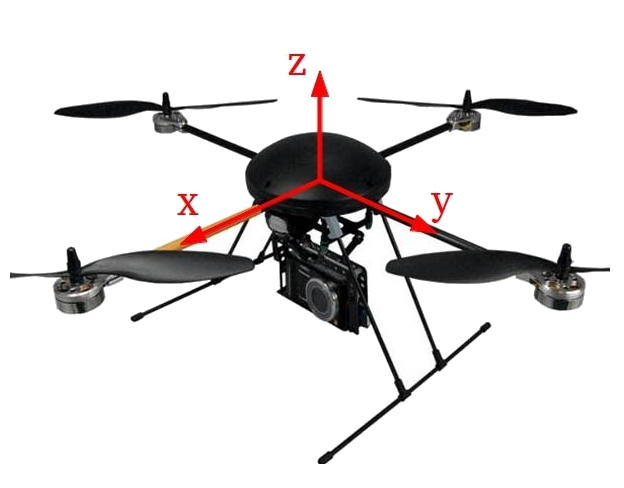
\includegraphics[width=0.4\textwidth]{./pics_sniffer/ejes_quad.jpg}
	\end{center}
	\vspace{-20pt}
	\caption{Definición de ejes}
	\label{fig:ejes_quad}
	\vspace{-70pt}
\end{wrapfigure}

Antes de presentar los resultados obtenidos en el proceso, se realiza una breve introducción al protocolo $i^2c$ y se presenta en la figura \ref{fig:ejes_quad} la definición de los ejes a utilizar, lo cual será de utilidad más adelante.

\newpage
\section{Introducción al protocolo $i^2c$}

El bus $i^2c$ es un bus de comunicaciones serie. Su nombre viene de \emph{Inter-Integrated Circuit} (Circuitos Inter-Integrados).\\
Utiliza dos líneas para transmitir la información: una para los datos y otra para la señal de reloj. Además será necesaria una tercera línea de tierra, como referencia.\\
En la imagen \label{fig:setup}\footnote{Imagen tomada de www.i2c-bus.org} se muestra un diagrama de un circuito equivalente simplificado de la conexión $i^2c$ entre 2 dispositivos.

\begin{figure}[h!]
	\centering
	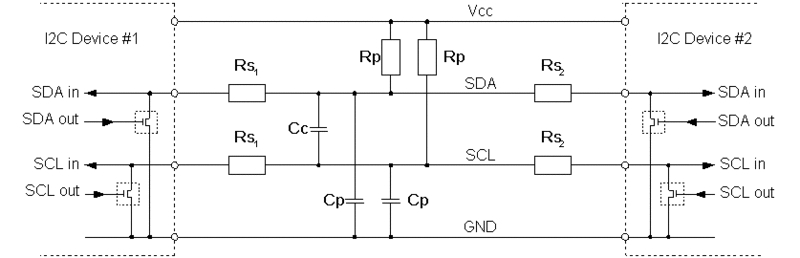
\includegraphics[width=0.8\textwidth]{./pics_sniffer/setup.jpg}
	\caption{Conexión $i^2c$.}
	\label{fig:setup}
\end{figure}
donde:
\begin{verbatim}
	Vcc	 Voltaje de entrada, típicamente varía entre 1.2 V y 5.5 V
	GND	 Tierra común
	SDA	 Línea serial de datos
	SCL	 Línea serial de reloj
	Rp 	 Resistencia de "Pull-up"
	Rs 	 Resistencia serie
	Cp 	 Capacitancia del cable
	Cc 	 Capacitancia de canal cruzado
\end{verbatim}

Las líneas \textbf{SDA} y \textbf{SCL} son de drenador abierto, lo que significa que tanto el maestro como los esclavos solamente pueden conducir a nivel bajo estas líneas o dejarlos abiertos. Si ningún dispositivo $i^2c$ está conduciendo hacia abajo la línea, la resistencia de \emph{pull-up} $R_p$ se encarga de conducir la línea a $V_{cc}$.\\

Cada dispositivo tiene asignada una dirección que lo identifica. Para establecer una comunicación la secuencia típica empieza por el maestro enviando una secuencia de comienzo de conexión, seguida de la dirección del esclavo con el cual desea comunicarse. Seguidamente el maestro envía un bit que determina si la acción que desea realizar es escritura o lectura, a lo que el esclavo correspondiente responde con un bit de \emph{acknowledge} (\textbf{Ack}). Luego el maestro envía la dirección de memoria interna del esclavo donde debe ser almacenada la información enviada, y por último envía los datos. Para finalizar la conexión, el maestro envía una secuencia de fin de conexión.

\newpage
\section{Pruebas en régimen}

Como se dijo anteriormente, para realizar el proceso de ingeniería inversa se utilizó el cuadricóptero y un analizador lógico. La forma de operar es enviar comandos conocidos con el control remoto y analizar los datos que se cursan en las líneas del bus. En la figura \ref{fig:sniffing} se muestra una foto del proceso descripto.

\begin{figure}[h!]
	\centering
	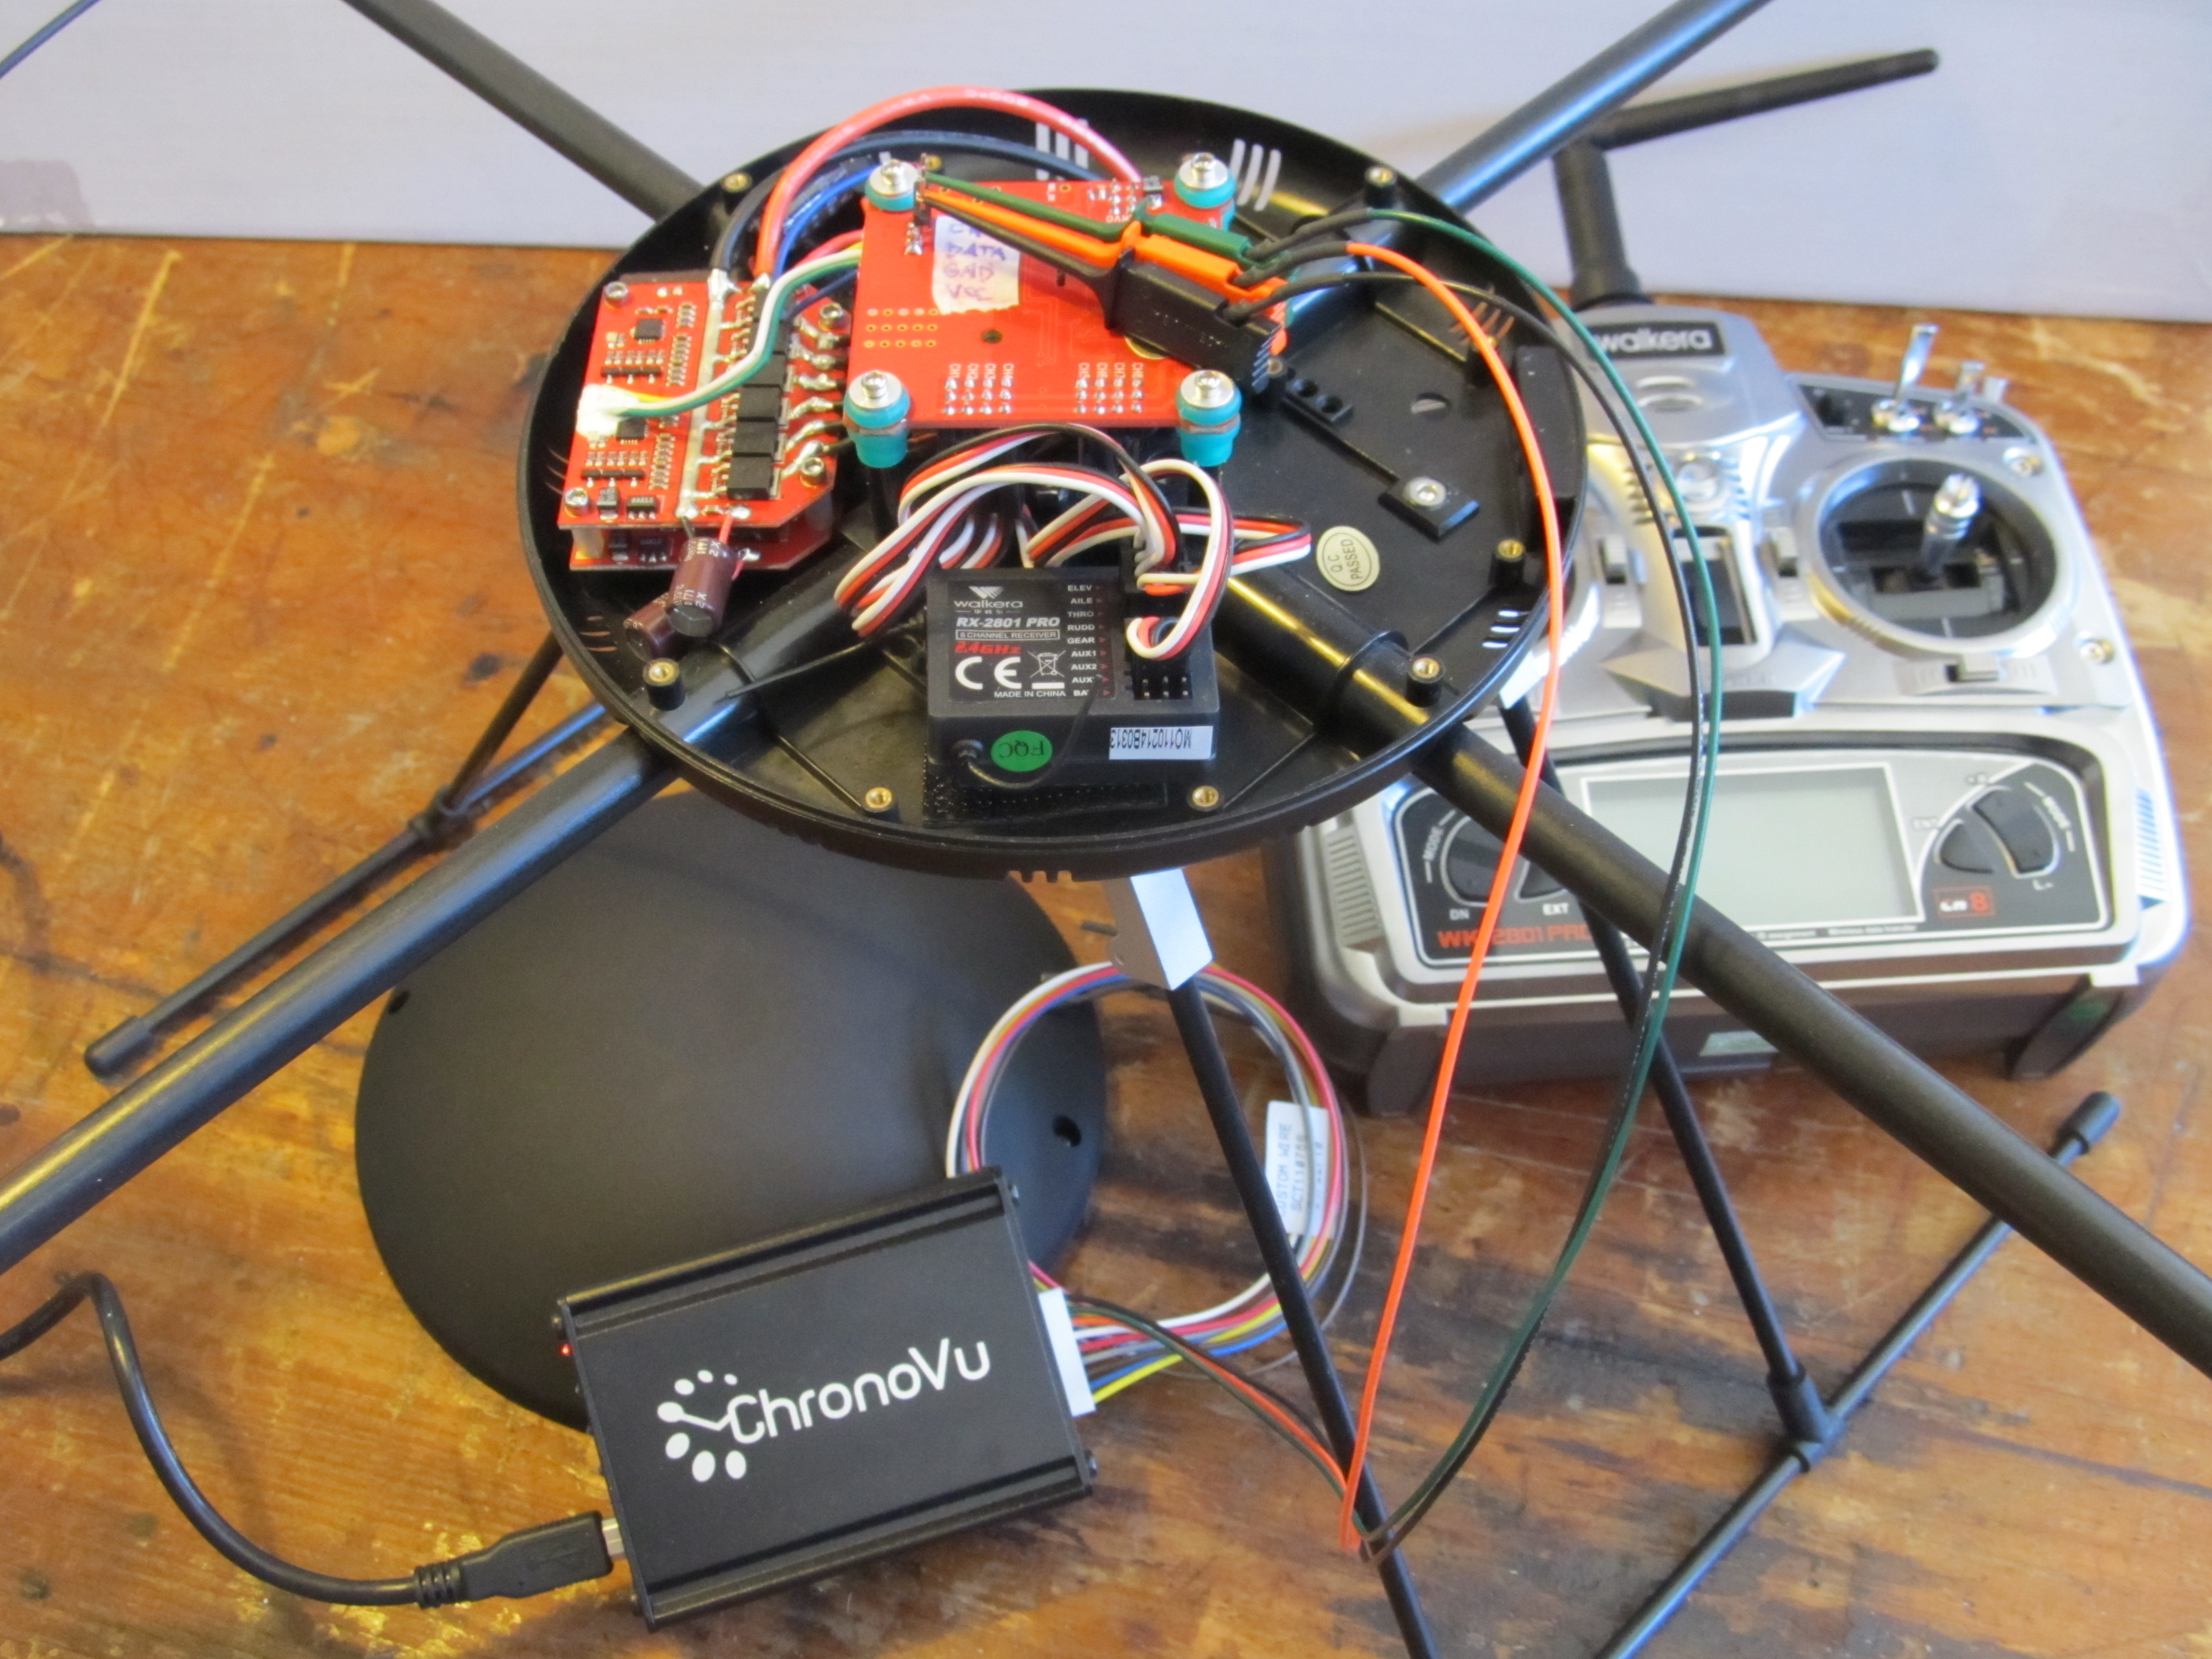
\includegraphics[width=0.6\textwidth]{./pics_sniffer/sniffing.jpg}
	\caption{Proceso de lectura del bus.}
	\label{fig:sniffing}
\end{figure}

Al realizar este proceso se puede observar que se repiten cada $2ms$ bloques similares al mostrado en la figura \ref{fig:bloque_snif}.

\begin{figure}[h!]
	\centering
	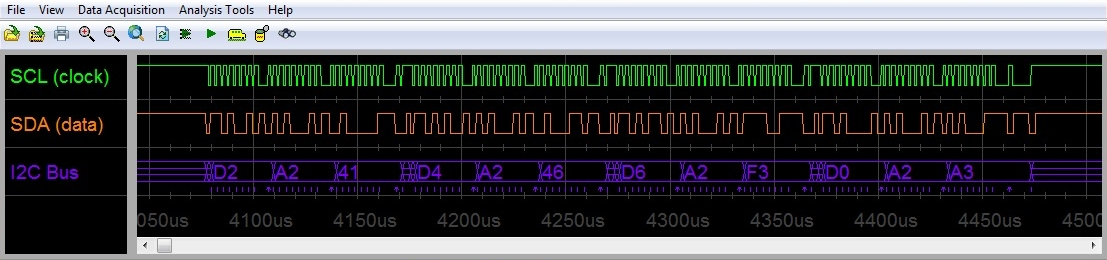
\includegraphics[width=1\textwidth]{./pics_sniffer/bloque_snif.jpg}
	\caption{Bloque de transmisión $i^2c$}
	\label{fig:bloque_snif}
\end{figure}

Rápidamente, visto lo anterior, se puede deducir que hay 4 esclavos correspondientes a los 4 ESC's de los 4 motores, cuyas direcciones en hexadecimal son \textbf{D0}, \textbf{D2}, \textbf{D4} y \textbf{D6}. La dirección de la memoria interna de los esclavos donde se almacenan los datos que envía el maestro es, en todos los casos \textbf{A2}. Además el maestro envía un tercer conjunto de datos que refiere, de alguna manera, a la velocidad con la que debe girar cada motor.
Este conjunto de órdenes, agrupadas por bloques como el que se muestra en la figura \ref{fig:bloque_snif}, se repite periódicamente, indicando la velocidad con la que debe girar cada motor.\\

Para comprender las pruebas realizadas es importante dejar en claro algunos aspectos previos. En la figura \ref{fig:tx} se muestra el transmisor utilizado para enviar comandos al cuadricóptero, un \textbf{Walkera WK-2801} y se indican los nombres de los mandos más importantes del mismo.


\begin{wrapfigure}{l}{0.55\textwidth}
	\vspace{-20pt}
	\begin{center}
	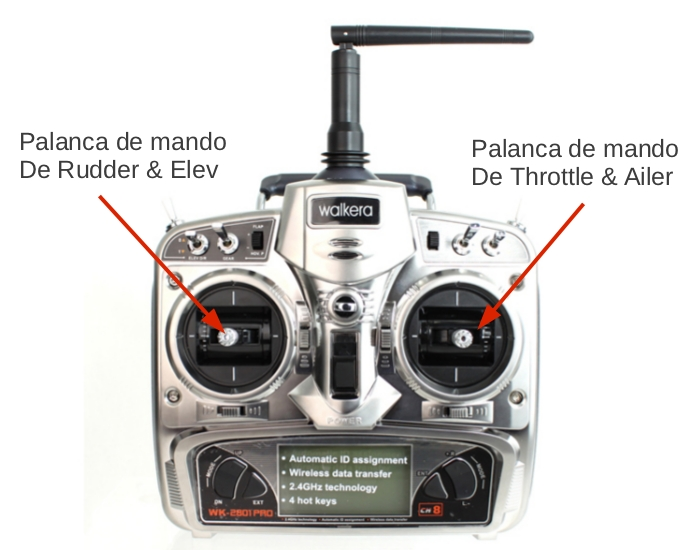
\includegraphics[width=0.45\textwidth]{./pics_sniffer/tx.jpg}
	\end{center}
	\vspace{-25pt}
	\caption{Transmisor}
	\label{fig:tx}
	\vspace{20pt}
\end{wrapfigure}

Al mover el mando de la izquierda (\textbf{Elev/Rudder}) en la dirección vertical (\textbf{Elev}) se logra que el cuadricóptero se eleve verticalmente, dando igual potencia a todos los motores, mientras que al moverlo en la dirección horizontal, el cuadricóptero presenta un movimiento de rotación según su eje vertical (que pasa por el centro).\\

Al mover el mando de la derecha (\textbf{Throttle/Aile}) en la dirección horizontal (\textbf{Aile}) y vertical (\textbf{Throttle}), se logran movimientos de rotación según los ejes horizontales \emph{x} e \emph{y} del cuadricóptero. Las definiciones de los ejes se pueden ver en la figura \ref{fig:ejes_quad}.\\

Se analizan las siguientes situaciones:
\begin{table}[H]
\begin{center}
\begin{tabular}{|p{30pt}|c|c|c|c|p{130pt}|} 
\hline \cellcolor[gray]{0.8} \centering \textbf{Id} & \cellcolor[gray]{0.8} \textbf{Elev} & \cellcolor[gray]{0.8} \textbf{Ruddle} & \cellcolor[gray]{0.8} \textbf{Aile} & \cellcolor[gray]{0.8} \textbf{Throttle} & \cellcolor[gray]{0.8} \textbf{Movimiento}  \\ \hline
\centering 0 & atrás& medio & medio & medio & idle \\ \hline
\centering 1 & medio & medio & medio & medio & vertical hacia arriba con aceleración constante \\ \hline
\centering 2 & adelante & medio & medio & medio & vertical hacia arriba con aceleración constante \\ \hline
\centering 3 & medio & izquierda & medio & medio & giro según eje $z$ \\ \hline
\centering 4 & medio & derecha & medio & medio &  giro según eje $-z$ \\ \hline
\centering 5 & medio & medio & izquierda & medio & giro según eje $-x$  \\ \hline
\centering 6 & medio & medio & derecha & medio & giro según eje $x$  \\ \hline
\centering 7 & medio & medio & medio & atrás & giro según eje $-y$  \\ \hline
\centering 8 & medio & medio & medio & adelante & giro según eje $y$  \\ \hline
\end{tabular} 
\end{center}
\caption{Pruebas realizadas}
\label{tab:pruebas}
\end{table}

Se realiza un análisis de los resultados obtenidos para cada motor, graficando el contenido del byte de datos que se le transmite a cada motor. Se obtienen representaciones como la mostrada en la figura \ref{fig:grafica_motores}

\begin{figure}[h!]
	\centering
	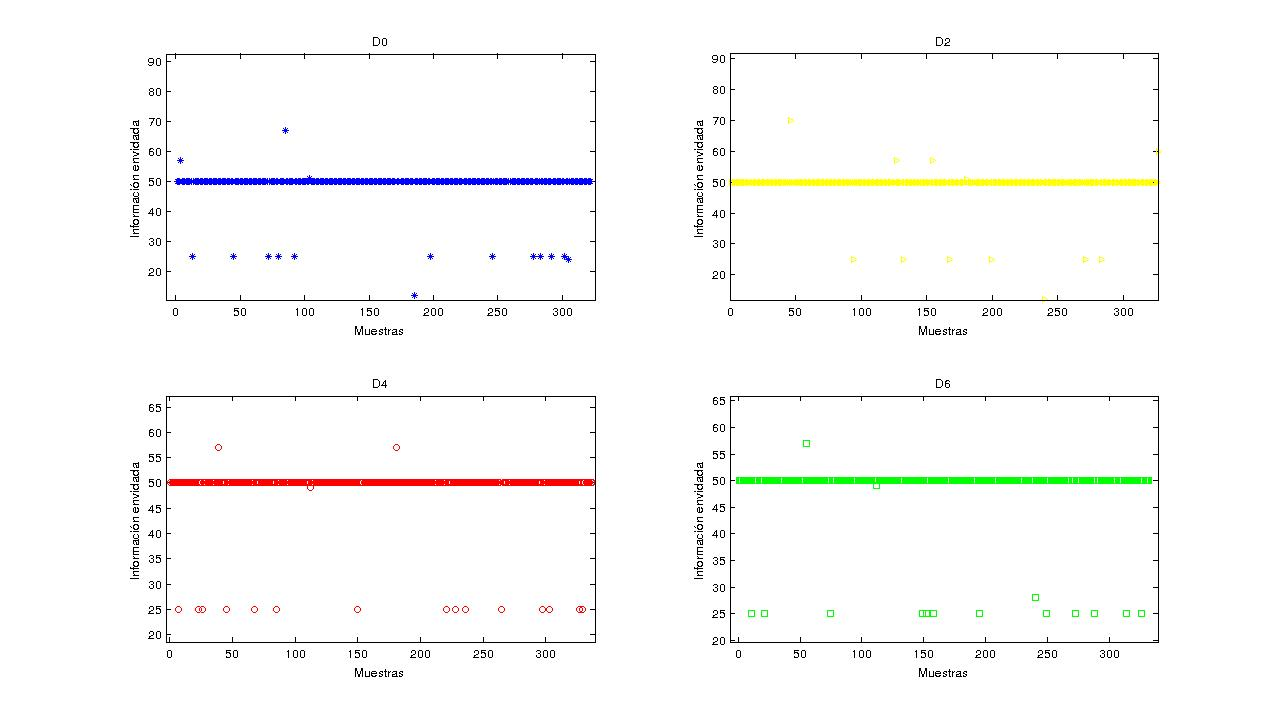
\includegraphics[width=1\textwidth]{./pics_sniffer/grafica_ejemplo.jpg}
	\caption{Prueba N$^o$ $0$}
	\label{fig:grafica_motores}
\end{figure}

En la figura \ref{fig:grafica_motores} se puede observar que a los 4 motores les llega un byte con el valor promedio en $50$, el cual corresponde a la mínima potencia entregada a los motores para encenderlos.\\

Haciendo un análisis similar con el resto de las pruebas detalladas en la tabla \ref{tab:pruebas} se construye la tabla \ref{tab:resumen_snif} donde se muestran los valores enviados a cada motor en promedio en todas las pruebas.\\

\begin{table}[H]
\begin{center}
\begin{tabular}{c|c|c|c|c|c|} 
\cline{2-5}
& \multicolumn{4}{c|}{\cellcolor[gray]{0.8} Valor promedio} \\ \hline
\multicolumn{1}{|c|}{\cellcolor[gray]{0.8} Prueba} & \cellcolor[gray]{0.8} D0 & \cellcolor[gray]{0.8} D2 & \cellcolor[gray]{0.8} D4 & \cellcolor[gray]{0.8} D6 & \cellcolor[gray]{0.8} Movimiento \\ \hline
\multicolumn{1}{|c|}{\cellcolor[gray]{0.8}0} & 50 & 50 & 50 & 50 & Idle \\ \hline
\multicolumn{1}{|c|}{\cellcolor[gray]{0.8}1} & 80 & 140 & 180 & 140 & $a_z=cte\neq 0$\\ \hline
\multicolumn{1}{|c|}{\cellcolor[gray]{0.8}2} & 180 & 220 & 250 & 240 & $a_z=cte\neq 0$ \\ \hline \hline
\multicolumn{1}{|c|}{\cellcolor[gray]{0.8}3} & 160 & 70 & 60 & 250 & giro según eje $z$ \\ \hline
\multicolumn{1}{|c|}{\cellcolor[gray]{0.8}4} & 50 & 200 & 200 & 100 & giro según eje $-z$\\ \hline \hline
\multicolumn{1}{|c|}{\cellcolor[gray]{0.8}5} & 250 & 160 & 140 & 50 & giro según eje $-x$\\ \hline
\multicolumn{1}{|c|}{\cellcolor[gray]{0.8}6} & 50 & 160 & 150 & 250 & giro según eje $x$ \\ \hline
\multicolumn{1}{|c|}{\cellcolor[gray]{0.8}7} & 90 & 50 & 250 & 160 & giro según eje $-y$\\ \hline
\multicolumn{1}{|c|}{\cellcolor[gray]{0.8}8} & 110 & 250 & 50 &  100 & giro según eje $y$\\ \hline
\end{tabular} 
\caption{Resumen de los resultados obtenidos}
\label{tab:resumen_snif}
\end{center}
\end{table}

De dicha tabla se pueden sacar algunas conclusiones que se analizarán en la sección \ref{sec:conclu};

\section{Prueba de arranque}
\label{sec:arranque}

En esta sección se analiza la secuencia de arranque del cuadricóptero, para obtener conclusiones sobre la misma. Se parte con la palanca de elevación al mínimo y se procede a moverla para hacer arrancar los motores.\\

Mientras la palanca de elevación se mantiene al mínimo, se le envía el valor 0 a los cuatro motores. Al mover la palanca, luego de un \emph{tiempo muerto} donde las líneas quedan inactivas, se les empieza a mandar el valor correspondiente a cada motor, como se puede ver en la figura \ref{fig:snif_arranque_lejos}.

\begin{figure}[h!]
	\centering
	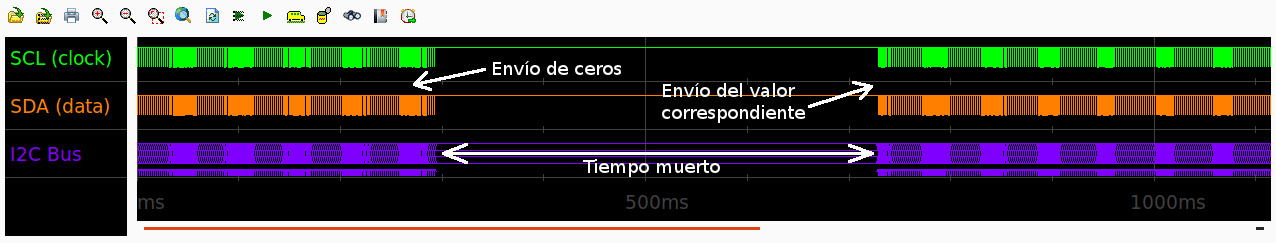
\includegraphics[width=1\textwidth]{./pics_sniffer/snif_arranque_lejos.png}
	\caption{Arranque}
	\label{fig:snif_arranque_lejos}
\end{figure}

Observando más detenidamente los comandos enviados se pueden sacar algunas conclusiones importantes. En la gran mayoría de los casos se envían los comandos en el orden $D2\rightarrow D4\rightarrow D6\rightarrow D0$ y se guardan en el registro 0xA2 del esclavo. Pero se puede observar una importante diferencia en la el último comando que se manda a cada motor antes de arrancar, es decir, el último comando en la tanda de ceros mostrada en la figura \ref{fig:snif_arranque_lejos}. En la figura \ref{fig:snif_arranque_ceros} se muestra una tanda regular de ceros y en la figura \ref{fig:snif_arranque_ultimos_ceros} se muestra la última tanda de ceros mencionada.\\

\begin{figure} [h!]
\centering
  \subfloat[Tanda normal de ceros]{\label{fig:snif_arranque_ceros}
  		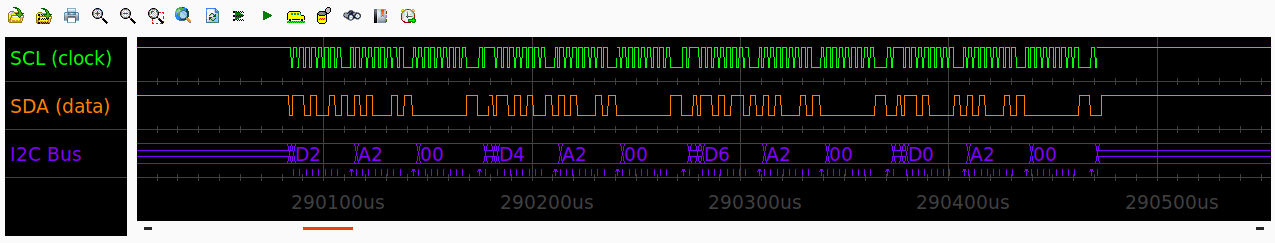
\includegraphics[width=1\textwidth]{./pics_sniffer/snif_arranque_ceros.png}} \\
  \subfloat[Última tanda de ceros]{\label{fig:snif_arranque_ultimos_ceros} 
  		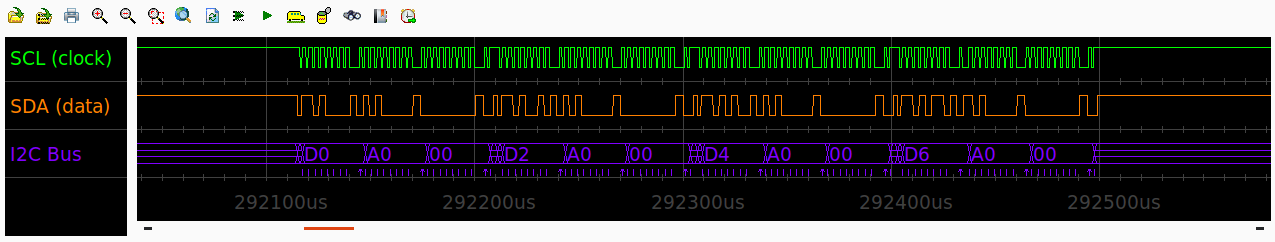
\includegraphics[width=1\textwidth]{./pics_sniffer/snif_arranque_ultimos_ceros.png}}
  \caption{Envío de ceros}
  \label{fig:snif_arranque_cerca}
\end{figure}

Se observan 2 claras diferencias:
\begin{itemize}
\item \textbf{El orden en el que se envían datos a los motores no es mismo} que el anterior. En este caso el orden es: $D0\rightarrow D2\rightarrow D4\rightarrow D6$.
\item \textbf{El registro en el que se escriben los datos es 0xA0}
\end{itemize}

Dichas diferencias se pueden observar claramente al graficar todos los datos obtenidos, como se muestra en la figura \ref{fig:arranque}. Se grafica para cada motor el valor que le llega (figura \ref{fig:arranque_val}) y el registro donde el valor es escrito (figura \ref{fig:arranque_reg}). Al analizar los resultados gráficamente resulta evidente el cambio en el registro al terminar de mandar los ceros. En la figura \ref{fig:arranque_val} se puede observar que el último cero que se manda a los motores, se manda alrededor de la muestra 150. Analizando la figura \ref{fig:arranque_reg} es clarísimo que alrededor de la muestra 150, el registro al que se envían los comandos cambia al valor 160 (0xA0), tal como se había observado anteriormente.

\begin{figure} [h!]
\centering
  \subfloat[Valores enviados a los motores]{\label{fig:arranque_val}
  		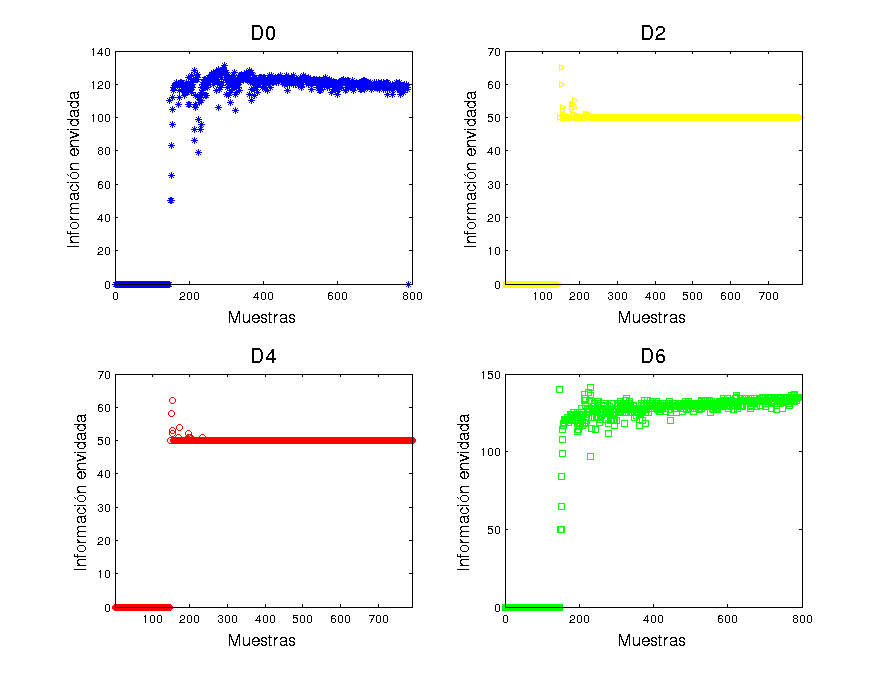
\includegraphics[width=.5\textwidth]{./pics_sniffer/arranque_val.png}}
  \subfloat[Registro al que se envía el valor]{\label{fig:arranque_reg} 
  		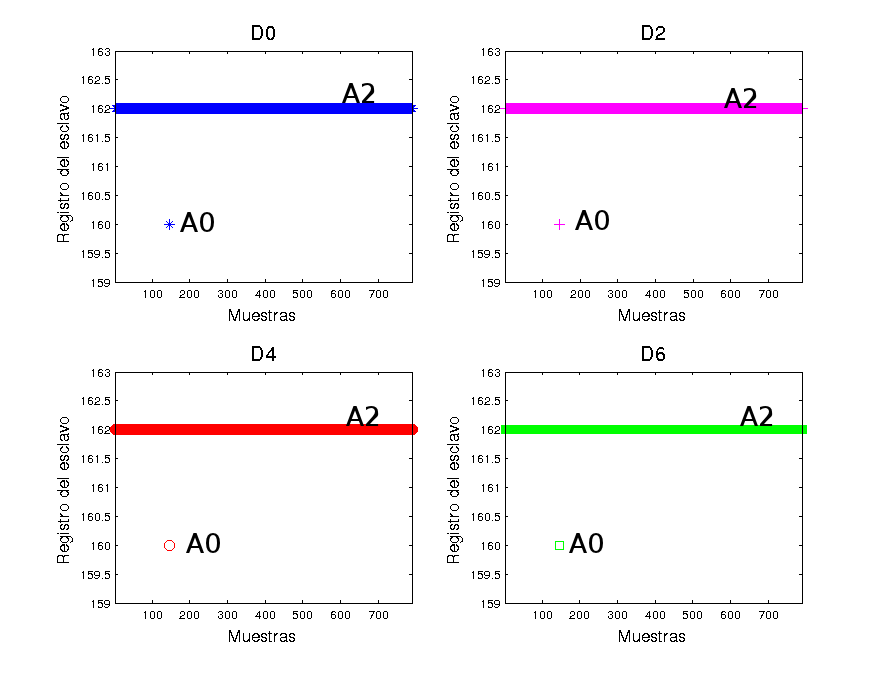
\includegraphics[width=.5\textwidth]{./pics_sniffer/arranque_reg.png}}
  \caption{Arranque}
  \label{fig:arranque}
\end{figure}


\section{Prueba de frenado}
\label{sec:frenado}
Se procede del mismo modo que en la prueba anterior (sección \ref{sec:arranque}), analizando los comandos enviados a los motores a la hora de apagarlos. Se realiza una prueba análoga a la anterior partiendo de los motores funcionando y bajando al mínimo la palanca de elevación, causando que estos se detengan.\\

Una vez que se lleva la palanca de elevación al mínimo, los motores se apagan y se permanece enviando ceros a los motores en el orden $D2\rightarrow D4\rightarrow D6\rightarrow D0$. Se pueden sacar algunas conclusiones importantes de la última tanda de valores distintos de cero enviados, mostrada en la figura \ref{fig:snif_frenado}:
\begin{itemize}
\item \textbf{El orden en el que se envían datos es $D0\rightarrow D2\rightarrow D4\rightarrow D6$}
\item \textbf{El registro en el que se escriben los datos es 0xA1}
\end{itemize}

\begin{figure}[h!]
	\centering
	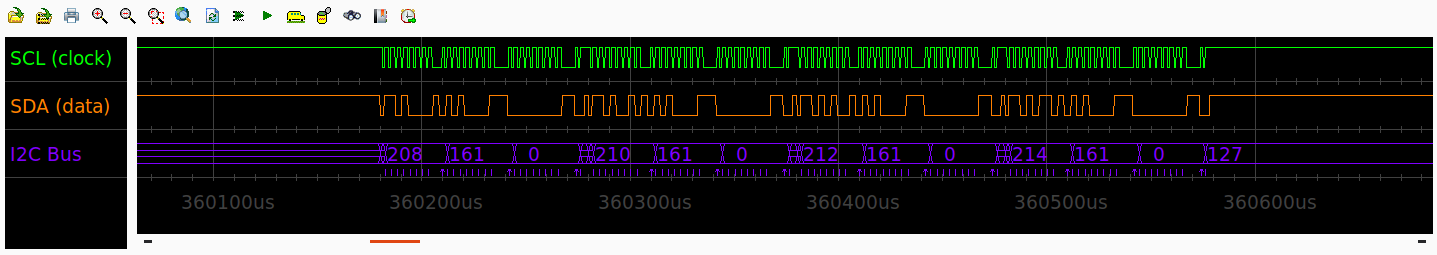
\includegraphics[width=1\textwidth]{./pics_sniffer/snif_frenado.png}
	\caption{Frenado}
	\label{fig:snif_frenado}
\end{figure}

Se presenta también un análisis gráfico en la figura \ref{fig:frenado}. En este caso, a diferencia del de la sección \ref{sec:arranque}, no es posible divisar con claridad el registro 0xA1 (161) en la figura \ref{fig:frenado_reg}, ya que se escriben comandos a una cantidad importante de registros diferentes.\\

\begin{figure} [h!]
\centering
  \subfloat[Valores enviados a los motores]{\label{fig:frenado_val}
  		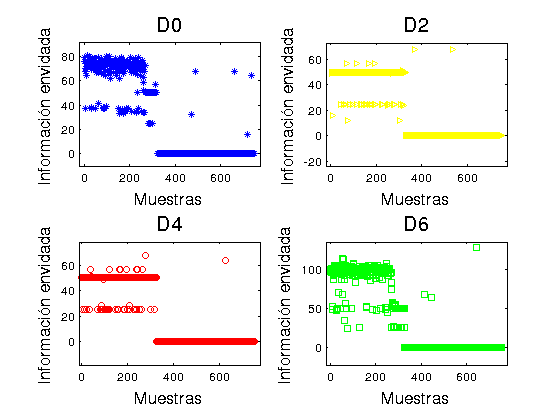
\includegraphics[width=.5\textwidth]{./pics_sniffer/frenado_val.png}}
  \subfloat[Registro al que se envía el valor]{\label{fig:frenado_reg} 
  		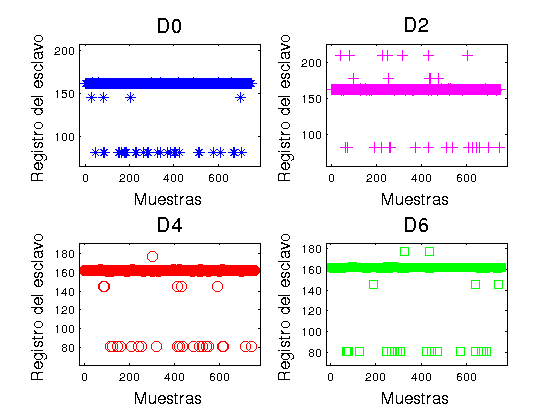
\includegraphics[width=.5\textwidth]{./pics_sniffer/frenado_reg.png}}
  \caption{Frenado}
  \label{fig:frenado}
\end{figure}

Avalados por la prueba realizada en la sección \ref{sec:MSP} que se verá luego, se afirma que en realidad la aparición de estos registros (por ejemplo los números 81, 145, etc) son causados por el proceso de \emph{sniffeo} y no son, de hecho, el comando mandado a los motores.\\

Analicemos por ejemplo el valor 81. Es claro que el resultado de dividir el valor 162 (correspondiente al conocido registro 0xA2) es exactamente 81, por lo cual parece probable que haya sido generado por un error del \emph{sniffer}, ya que un corrimiento hacia la derecha de un bit en una palabra binaria es equivalente a realizar una división entre 2. Es probable entonces que el sniffer haya incluido un bit en 0 antes de la verdadera palabra y haya descartado el último bit, causando una aparente división entre 2. Más graficamente:\\

\begin{center} 162 = 10100010 $\rightarrow$ \color{green}0\color{black}1010001\color{red}\xcancel{0}\color{black} = 81\\
\end{center}

En verde se muestra el bit agregado y en rojo el eliminado.

\section{Conclusiones}
\label{sec:conclu}

\begin{itemize}
\item La comunicación entre el amo y los esclavos por medio del protocolo $i^2c$ se lleva a cabo mediante un  formato del tipo \begin{verbatim} Dirección esclavo - Lugar de memoria donde guardar dato - dato \end{verbatim}
\item Dicho formato se repite para todos los esclavos
\item Cada esclavo recibe una actualización de estado (un dato nuevo) cada $2 ms$
\item La velocidad mínima de funcionamiento se logra enviando el valor 50
\item La velocidad máxima de funcionamiento se logra enviando el valor 250
\item Cuando el mando de Elevación del control se encuentra al mínimo, se les envía el valor 0 a los cuatro motores periódicamente con el formato mencionado.
\item La dirección de memoria interna de todos los esclavos donde se guardan los datos recibidos por el maestro es siempre 0x$A2$ (ó $162$), a excepción del arranque y el frenado.
\item El último comando enviado antes de arrancar se guarda en el registro 0xA0.
\item El último comando enviado antes de frenar se guarda en el registro 0xA1.
\item El orden normal en el que se envían los comandos es $D2\rightarrow D4\rightarrow D6\rightarrow D0$, menos en los casos descriptos en los 2 puntos anteriores donde el orden es $D0\rightarrow D2\rightarrow D4\rightarrow D6$.
\item La correspondencia entre las direcciones y los motores se muestra en la figura \ref{fig:correspondencias}. El motor con dirección 0xD0 es el de adelante, el motor con dirección 0xD4 es el de atrás y mirándolo de frente el de la izquierda se corresponde con 0xD0, y el de la derecha con 0xD6
\item Las direcciones 0xD0, 0xD2, 0xD4 y 0xD6 (de 8 bits) en realidad no refieren únicamente a direccionamiento, sino que incluyen además el bit de lectura/escritura, por lo cual cada esclavo tendrá una única dirección de 7 bits. Notar que las direcciones 0xD0 a 0xD6 al pasarlas a binario todas terminan en 0, lo cual implica que se tratan de comandos de escritura. Al omitir el último bit se obtienen las direcciones (sin incluir el bit de lectura/escritura) como se puede ver a continuación:
\begin{eqnarray}
\mathrm{0xD0} (11010000) &\longrightarrow &\mathrm{0x68} (1101000) \\
\mathrm{0xD2} (11010010) &\longrightarrow &\mathrm{0x69} (1101001) \\
\mathrm{0xD4} (11010100) &\longrightarrow &\mathrm{0x6A} (1101010) \\
\mathrm{0xD6} (11010110) &\longrightarrow &\mathrm{0x6B} (1101011) 
\end{eqnarray}
Las direcciones de los motores son entonces: \textbf{0x68}, \textbf{0x69}, \textbf{0x6A}, \textbf{0x6B}.
\item En las pruebas 0, 1, 2, 5, 6 y 7 se observa que la suma del valor promedio enviado al motor D0 más el enviado a la dirección D2 es similar a la suma de los valores entregados a los motores con dirección D4 y D6, lo cual implica un equilibrio en los pares realizados en ambos sentidos. Se infiere entonces que el movimiento según el eje ``z" se logra desequilibrando los pares en ambos sentidos (según ``z'' y según ``-z'')
\end{itemize}

\begin{figure}[h!]
	\centering
	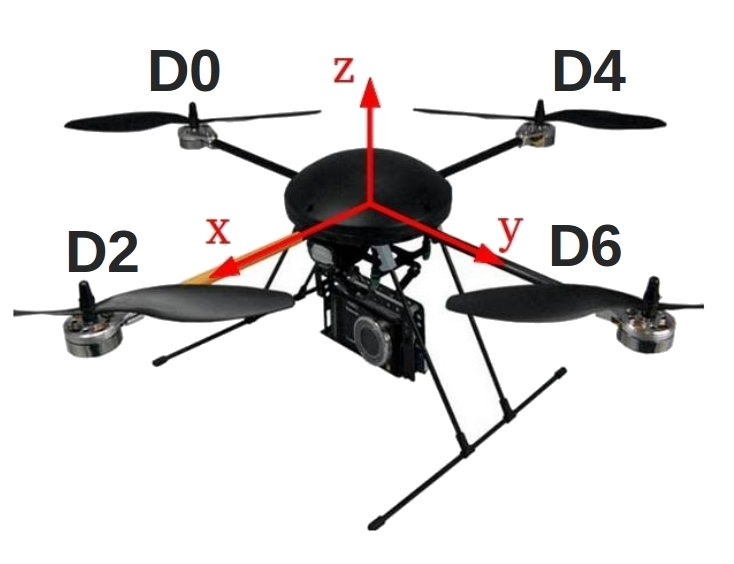
\includegraphics[width=0.4\textwidth]{./pics_sniffer/correspondencias.jpg}
	\caption{correspondencias}
	\label{fig:correspondencias}
\end{figure}

\section{Verificaciones}
Se presentan diversas verificaciones realizadas para corroborar la veracidad de las conclusiones sacadas, además de la corroboración experimental utilizando el puerto $i^2c$ de la Beagleboard.\\

\subsection*{i2cdetect}
Utilizando la librería \emph{i2c Tools}\footnote{http://www.lm-sensors.org/wiki/i2cToolsDocumentation} con la Beagleboard es posible mandar el comando \textbf{i2cdetect} que lo que hace es preguntar a todos los esclavos que estén presentes en el bus, por su dirección. El resultado en terminal es el siguiente
\begin{verbatim}
root@beagleboard:~# i2cdetect -r 2
WARNING! This program can confuse your I2C bus, cause data loss and worse!
I will probe file /dev/i2c-2 using read byte commands.
I will probe address range 0x03-0x77.
Continue? [Y/n] y

     0  1  2  3  4  5  6  7  8  9  a  b  c  d  e  f
00:          -- -- -- -- -- -- -- -- -- -- -- -- -- 
10: -- -- -- -- -- -- -- -- -- -- -- -- -- -- -- -- 
20: -- -- -- -- -- -- -- -- -- -- -- -- -- -- -- -- 
30: -- -- -- -- -- -- -- -- -- -- -- -- -- -- -- -- 
40: -- -- -- -- -- -- -- -- -- -- -- -- -- -- -- -- 
50: -- -- -- -- -- -- -- -- -- -- -- -- -- -- -- -- 
60: -- -- -- -- -- -- -- -- 68 69 6a 6b -- -- -- -- 
70: -- -- -- -- -- -- -- --
\end{verbatim}

Puede verse claramente que las direcciones de los esclavos obtenidas por la función mencionada son: \textbf{0x68}, \textbf{0x69}, \textbf{0x6A}, \textbf{0x6B}.

\subsection*{MSP430F5438}
\label{sec:MSP}
Se utiliza el chip \textbf{MSP430F5438}, que se muestra en la figura \ref{fig:MSP430F5438}.

\begin{wrapfigure}{r}{0.5\textwidth}
	\begin{center}
	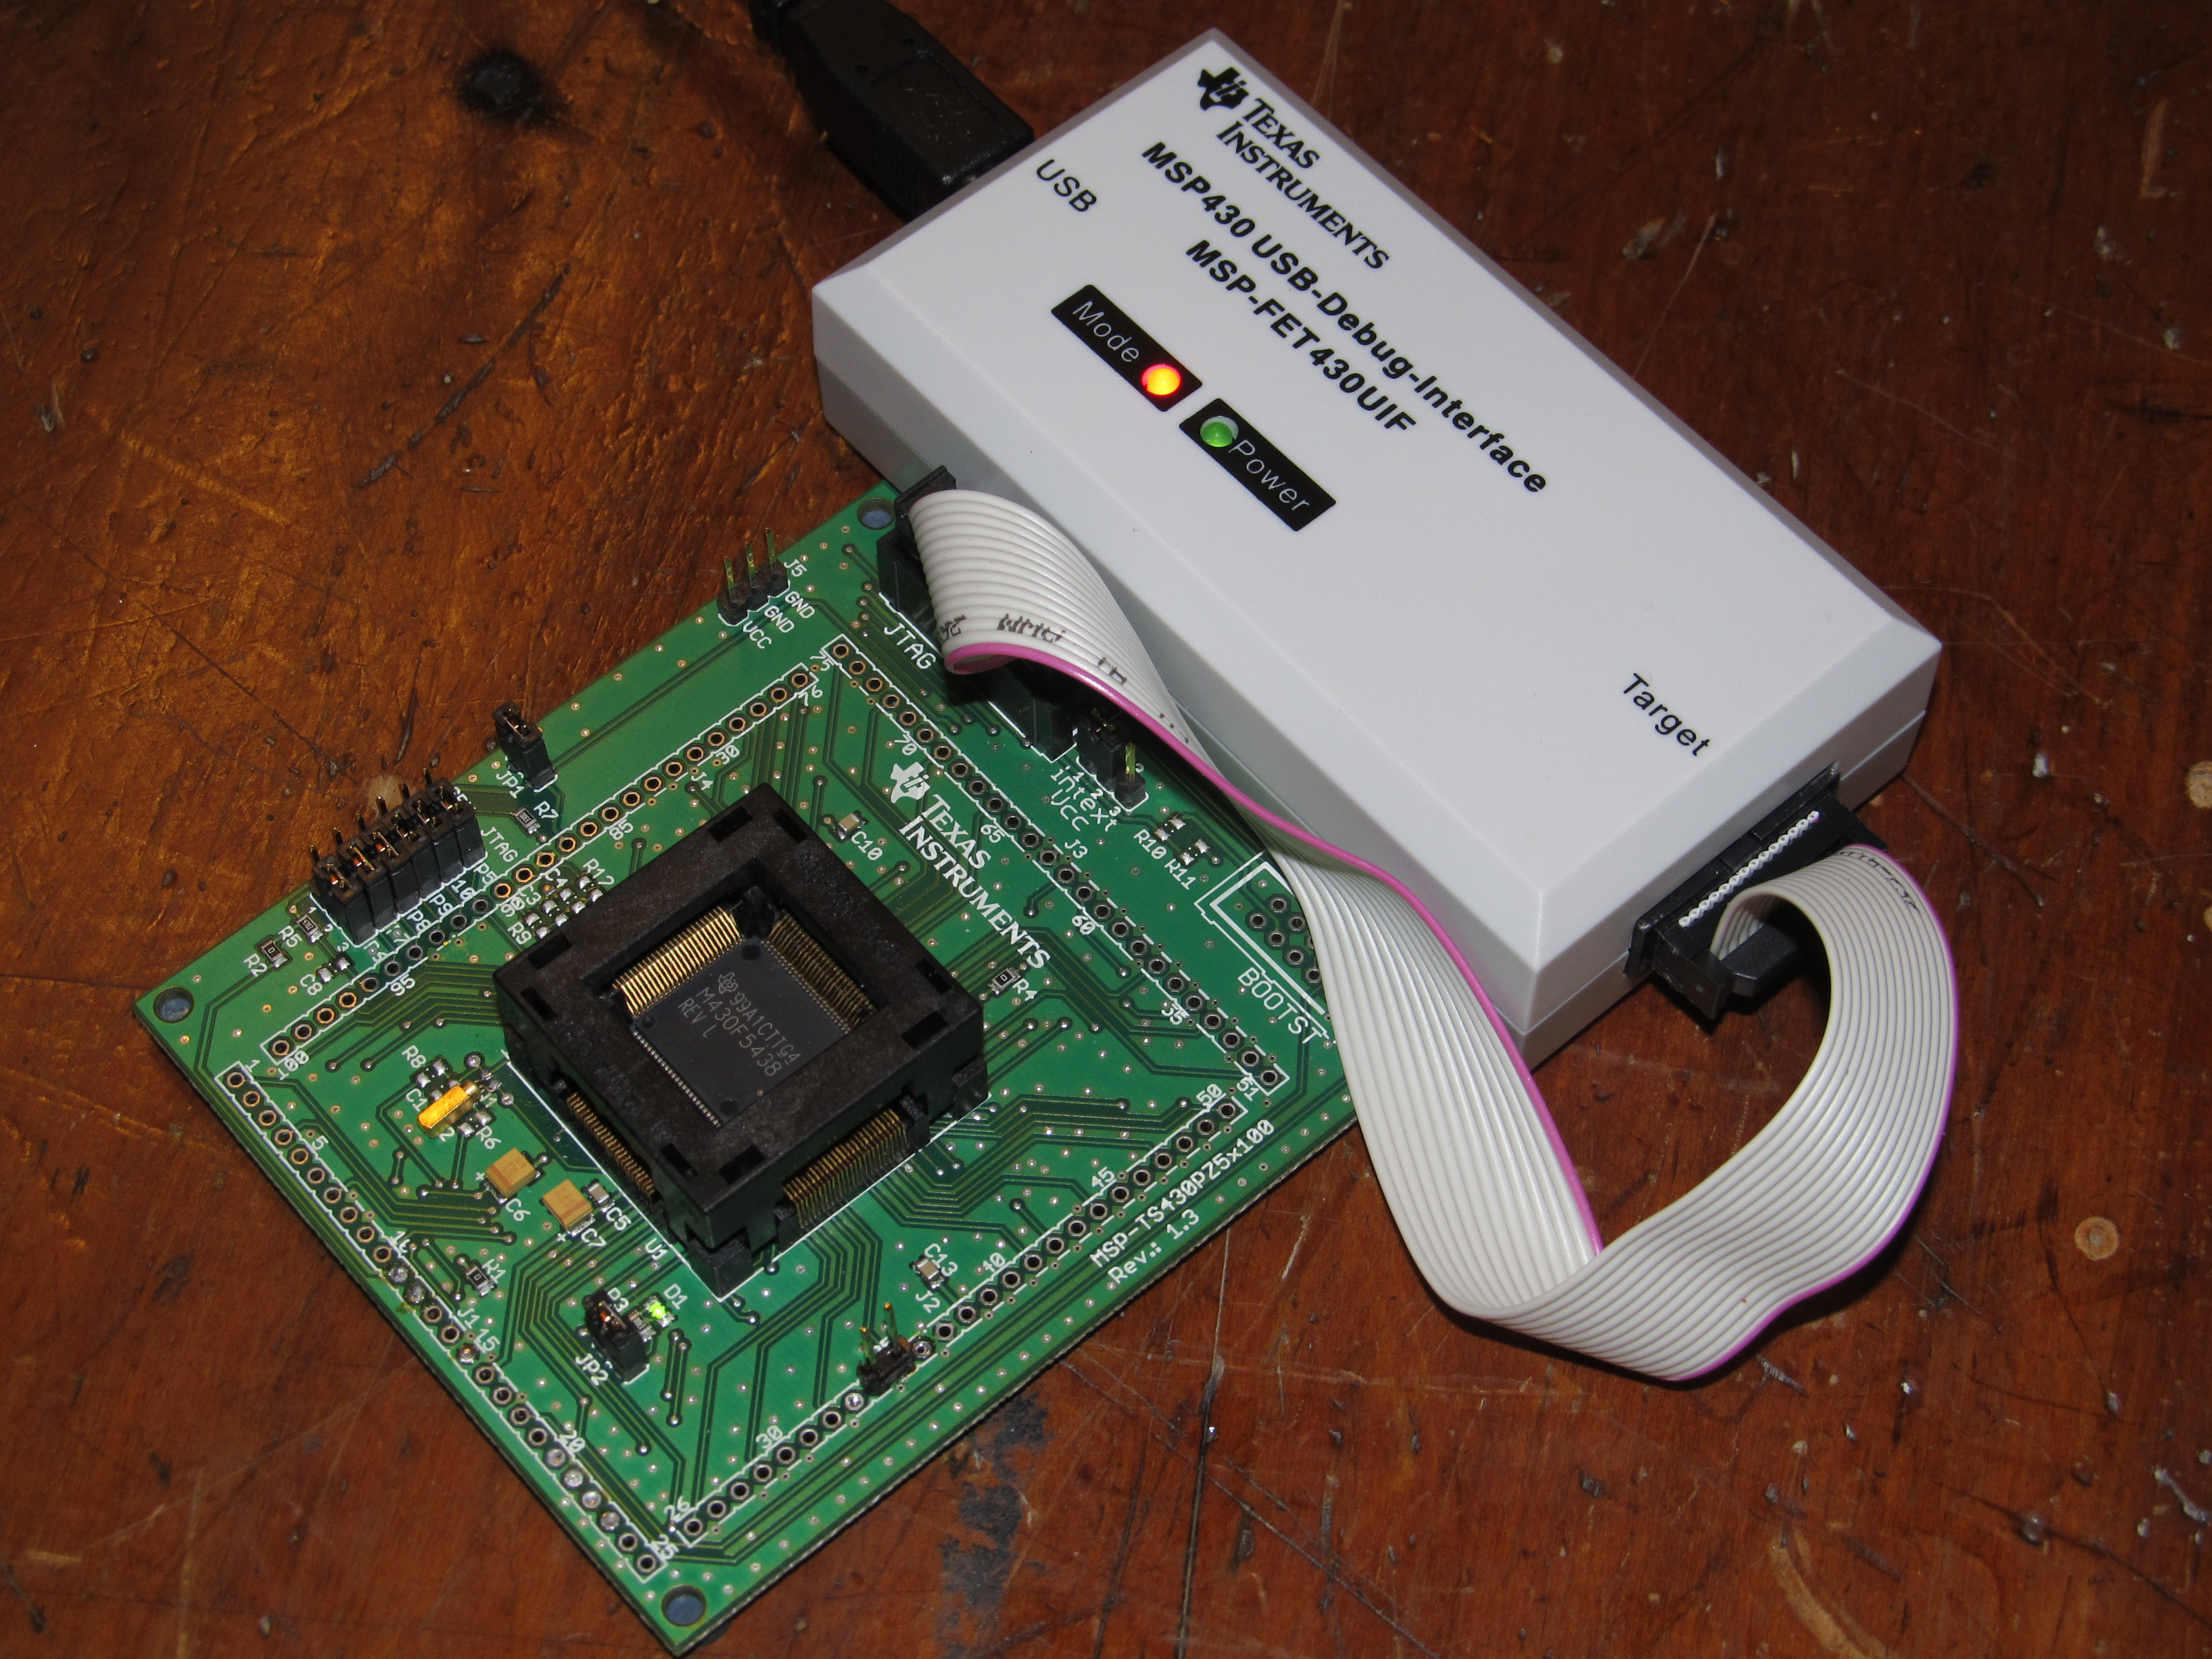
\includegraphics[width=0.4\textwidth]{./pics_sniffer/MSP430F5438.jpg}
	\end{center}
	\vspace{-20pt}
	\caption{MSP430F5438}
	\label{fig:MSP430F5438}
\end{wrapfigure}

El MSP430F5438 posee un puerto $i^2c$ habilitado para su utilización. Se configurara como esclavo y se guarda en una variable todos los comandos recibidos en el bus. De este modo se logra independizarse de los problemas que pueda introducir el sniffer y se obtiene exactamente el comando mandado a ese esclavo. Se le configura la dirección 0x68 para comunicarse con el maestro cuando éste mande comandos a esa dirección.\\

Luego, analizando la variable donde se guardan los comandos, es posible obtener información más concluyente.\\

En la figura \ref{fig:MSP_arranque} se muestran los resultados obtenidos al adquirir datos en un arranque.

\begin{figure} [h!]
\centering
  \subfloat[Valores enviados a los motores]{\label{fig:MSP_arranque_val}
  		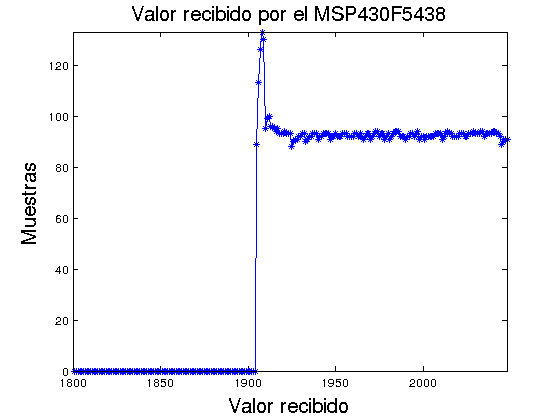
\includegraphics[width=.5\textwidth]{./pics_sniffer/MSP_arranque_val.png}}
  \subfloat[Registro al que se envía el valor]{\label{fig:MSP_arranque_reg} 
  		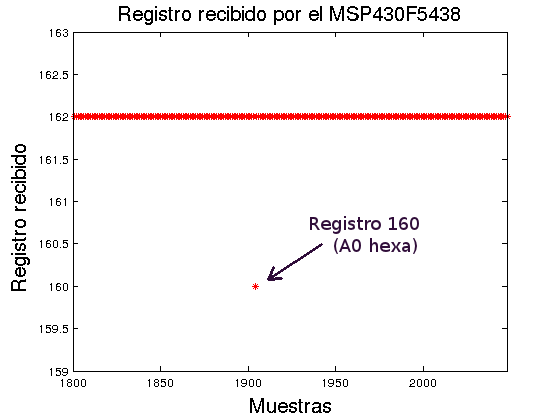
\includegraphics[width=.5\textwidth]{./pics_sniffer/MSP_arranque_reg.png}}
  \caption{Arranque detectado por el MSP430F5438}
  \label{fig:MSP_arranque}
\end{figure}

En la figura \ref{fig:MSP_frenado} se muestran los resultados obtenidos al adquirir datos en un frenado.

\begin{figure} [h!]
\centering
  \subfloat[Valores enviados a los motores]{\label{fig:MSP_frenado_val}
  		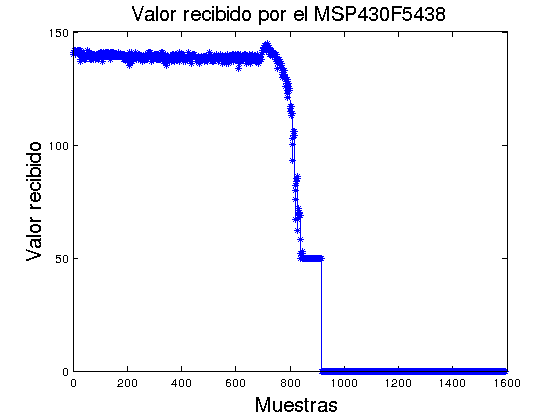
\includegraphics[width=.5\textwidth]{./pics_sniffer/MSP_frenado_val.png}}
  \subfloat[Registro al que se envía el valor]{\label{fig:MSP_frenado_reg} 
  		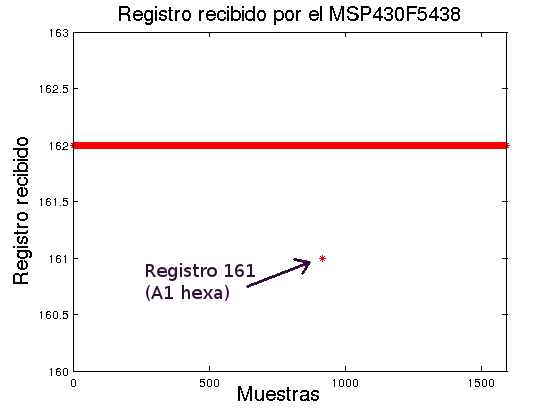
\includegraphics[width=.5\textwidth]{./pics_sniffer/MSP_frenado_reg.png}}
  \caption{Frenado}
  \label{fig:MSP_frenado}
\end{figure}

Estas últimas dos figuras son las corroboraciones más concluyentes que se obtuvieron. Ratifica y deja bien en claro lo antes dicho sobre los registros: \textbf{para el arranque se escribe en la dirección 0xA0 del esclavo y para el frenado se escribe en la dirección 0xA1.}\\

A su vez sirve de confirmación para los errores del sniffeado detectados en la sección \ref{sec:frenado}.





\end{document}